% override specific chktex warnings

% chktex-file 1 - ignore commands followed by a space, e.g. \\ new line here
% chktex-file 3 - enclose previous parentheses wit {}
% chktex-file 9 - sometimes messes up with ( and {
% chktex-file 36 - put a space in front of parentheses
% chktex-file 45 - don't use $$ instead of \[, etc
% chktex-file 46 - don't use $ instead of \(, etc

\documentclass[9pt,xcolor={svgnames, x11names},mathpazo, professionalfonts]{beamer}

\usepackage{amsmath}
\usepackage{amssymb}
\usepackage{graphicx}
\usepackage{booktabs}  % for top and bottom spacing in table cells
% \usepackage{mathpazo}
\usepackage{textcomp}
\usepackage{multirow}
\usepackage{cancel}
\usepackage{array}
%\usepackage{enumerate}
% \usepackage{enumitem} %causes compile error, stack size exceeded?
\usepackage{gensymb} % for \degree
\usepackage[many]{tcolorbox}
\usepackage{verbatim}
\usepackage{bm}
\usepackage{graphicx}
\usepackage{scalerel}
% \usepackage{svg}
\usepackage{tikz}
\usepackage{tkz-linknodes}
\usepackage[export]{adjustbox} % for tight borders around photos
\usepackage{pgf} % for sait logo in beamer
\usepackage{pgfmath}
\usepgfmodule{oo}
%\usetikzlibrary{shapes,decorations,shadows,calc}
\usetikzlibrary{shadows,calc,arrows.meta}
% \usetikzlibrary{decorations.shapes}
%\usetikzlibrary{shapes.callouts}
% bloody coils
\usetikzlibrary{decorations.pathmorphing}
\usetikzlibrary{shapes.multipart}

% counter for resuming enumerated list numbers
\newcounter{resumeenumi}
\newcommand{\suspend}{\setcounter{resumeenumi}{\theenumi}}
\newcommand{\resume}{\setcounter{enumi}{\theresumeenumi}}

\newcommand\lb{\linebreak}
\newcommand\pars{\par\smallskip}
\newcommand\parm{\par\medskip}
\newcommand\parb{\par\bigskip}

\makeatletter
\providecommand{\gettikzxy}[3]{%
	\tikz@scan@one@point\pgfutil@firstofone#1\relax
	\edef#2{\the\pgf@x}%
	\edef#3{\the\pgf@y}%
}
\makeatother



% full width colored block but color specifiable
%\cb[body bg strength]{header bg}{header text}{body text}
\newcommand{\cb}[4][15]{
	\setbeamercolor{block title}{bg = #2}
	\setbeamercolor{block body}{bg = #2!#1}
	\setbeamercolor{item projected}{bg=#2, fg=white}
	\begin{center}
		\begin{block}{#3}
			#4
		\end{block}
	\end{center}
}

% colored block with width specified
% \cbw[body bg strength]{header bg}{width}{header text}{body text}
\newcommand{\cbw}[5][15]{
	\begin{center}
		%\vspace{-0.35cm}
		\begin{minipage}{#3\textwidth}
			\setbeamercolor{block title}{bg= #2}
			\setbeamercolor{block body}{bg= #2!#1}
			\setbeamercolor{item projected}{bg=#2, fg=white}
			\begin{block}{#4}
				\raggedright
				#5
			\end{block}
		\end{minipage}
	\end{center}
}

% centered minipage with text \raggedright
%\cmini[width]{content}
\newcommand{\cmini}[2][0.8]{
	\begin{center}
		\begin{minipage}{#1\columnwidth}
			\raggedright
			#2
		\end{minipage}
	\end{center}
}

%left flushed minipage
\newcommand{\mini}[2][0.8]{
	\begin{minipage}{#1\columnwidth}
		\raggedright
		#2
	\end{minipage}
}

%left flushed minipage, top aligned
\newcommand{\minit}[2][0.8]{
	\begin{minipage}[t]{#1\columnwidth}
		\raggedright
		#2
	\end{minipage}
}

%left flushed minipage
% \newcommand{\miniT}[2][0.8]{
%  \begin{minipage}[T]{#1\columnwidth}
%   \raggedright
%   #2
%  \end{minipage}
% }

%left flushed minipage
\newcommand{\minib}[2][0.8]{
	\begin{minipage}[b]{#1\columnwidth}
		\raggedright
		#2
	\end{minipage}
}

\newcommand{\cfig}[2][1]{% centred, scaled graphic
	\begin{center}
		\includegraphics[scale=#1]{#2}
	\end{center}
}
% figure with tight border for photos
% \cfigb[saitMaroon]{borderwidth with unit}{scale}{image}
\newcommand{\cfigb}[4][structure]{
	% \usepackage{adjustbox}
	\setlength{\fboxrule}{1pt}
	\begin{center}
		\includegraphics[scale=#3, cframe= #1 #2]{#4}
	\end{center}
}

\newcommand{\imgbox}[3]{
	% \setlength{\fboxsep}{12pt}
	\includegraphics[scale=#1, cframe= structure #3]{#2}
}

% \imgboxbg[bg color=white]{scale}{path/to/img}{border color}{border, e.g. 2pt}{margin, e.g. 4pt}
\newcommand{\imgboxbg}[6][white]{
	\setlength{\fboxrule}{#5}
	\setlength{\fboxsep}{#6}
	\centering
	\fcolorbox{#4}{#1}{\includegraphics[scale=#2]{#3}}
}

\newcommand{\fig}[2][1]{% scaled graphic
	\includegraphics[scale=#1]{#2}
}

% centred framed  box black border
%\cbox[width]{content}
\newcommand{\cbox}[2][0.9]{% framed centered  box
	\setlength\fboxsep{0.042\columnwidth}
	\setlength\fboxrule{0.0015\columnwidth}
	\begin{center}
		\fcolorbox{black}{white}{
			\vspace{-0.5cm}
			\begin{minipage}{#1\columnwidth}
				\raggedright
				#2
			\end{minipage}
		}
	\end{center}
	\setlength\fboxsep{0cm}
}



\newtcolorbox{mybox}[1][]
{
	colback=white,
	top=0.25cm,
	bottom=0.25cm,
	left=0.25cm,
	right=0.25cm,
	colframe=structure,
	fonttitle=\bfseries,
	enhanced, drop fuzzy shadow,
	% attach boxed title to top left={yshift=-2mm, xshift=5mm},
	attach boxed title to top left={yshift=-2mm, xshift=5mm}, colbacktitle=structure!80!white, #1}

\newtcolorbox{plainbox}[1][]{colback=white, sharp corners, top=0.125cm, bottom=0.125cm, left=0pt, right=0pt, boxrule=0.5pt,colframe=structure,fonttitle=\bfseries, colbacktitle=structure, arc=0mm, #1}
%
\newtcbtheorem{myexam}{Example}%
{
	enhanced,
	colback=white,
	top=0.375cm,
	bottom=0.25cm,
	left=0.375cm,
	right=0.375cm,
	colframe=structure,
	fonttitle=\bfseries,
	drop fuzzy shadow,
	%description font=\mdseries\itshape,
	attach boxed title to top left={yshift=-2mm, xshift=5mm},
	colbacktitle=structure!80!white
	}{exam}% then \pageref{exer:theoexample} references the theo

\newcommand{\myexample}[2][red]{
	% \tcb\tcbset{theostyle/.style={colframe=red,colbacktitle=yellow}}
	\begin{myexam}{}{}
		\raggedright
		#2
	\end{myexam}
	% \tcbset{colframe=structure,colbacktitle=structure}
}

\newtcbtheorem{myexer}{Exercise}%
{
	enhanced,
	colback=white,
	top=0.375cm,
	bottom=0.25cm,
	left=0.375cm,
	right=0.375cm,
	colframe=structure,
	fonttitle=\bfseries,
	drop fuzzy shadow,
	%description font=\mdseries\itshape,
	attach boxed title to top left={yshift=-2mm, xshift=5mm},
	colbacktitle=structure!80!white
	}{exer}

\newcommand{\myexercise}[2][red]{
	% \tcb\tcbset{theostyle/.style={colframe=red,colbacktitle=yellow}}
	\begin{myexer}{}{}
		\raggedright
		#2
	\end{myexer}
	% \tcbset{colframe=structure,colbacktitle=structure}
}

\input{../../Includes/definedColors}
% override specific chktex warnings
% chktex-file 46 - don't use $ instead of \(, etc)
% chktex-file 36 - don't require space in front of parenthesis
% chktex-file 37 - don't require space in front of parenthesis
% chktex-file 26 - don't require space in front of punctuation
% chktex-file 1 - ignore commands followed by a space, e.g. \\ new line here
% chktex-file 9 - sometimes messes up with ( and {

\begin{comment}
Shadings are useful to give the illusion of 3D in examples and exercises presented to engineering technology students.
Vertical and horizontal shadings of rectangles are fairly straightforward to produce with the shading library included in
a recent build of Tikz.
Rotation of shaded squares is also intuitive, but rotation of a shaded rectangle appears to be both a function of the specified
rotation angle and the length to width ratio of the rectangle. This makes aligning the shading of a rotated rectangle's
fill with the stroke of a rotated rectangle a bit of an inelegant trial-and-error exercise (for me, at any rate).


\end{comment}

%http://tex.stackexchange.com/questions/33703/extract-x-y-coordinate-of-an-arbitrary-point-in-tikz
\makeatletter
\providecommand{\gettikzxy}[3]{%
	\tikz@scan@one@point\pgfutil@firstofone#1\relax
	\edef#2{\the\pgf@x}%
	\edef#3{\the\pgf@y}%
}
\makeatother


%%%%%%%%%%%%%%%%%%%%%%%%%%%%%%%% A CLASS FOR ROTATED RECTANGLES WITH A SHADED FILL %%%%%%%%%%%%%%%%%%%%%%%%%%%%%%%%%%%%%%%%
\pgfooclass{rrect}{
	% the following should be set in the calling program: \hi, \radii, \extend
	% Ax, Ay, Bx, By, outershade, innershade
	\method rrect(#1,#2,#3,#4,#5,#6) { % The constructor; everything is done in here
		\def\Ax{#1} \def\Ay{#2} \def\Bx{#3} \def\By{#4} \def\outercolor{#5} \def\innercolor{#6}
		\pgfmathparse{\Bx-\Ax} \let\deltaX\pgfmathresult
		\pgfmathparse{\By-\Ay} \let\deltaY\pgfmathresult
		\ifthenelse{\equal{\deltaX}{0.0}}
		{	% vertical rod is a special case; otherwise atan gets a div by 0 error
			\pgfmathparse{\By>\Ay} \let\ccw\pgfmathresult
			\ifthenelse{\equal{\ccw}{1}}{%
				\def\rot{90}}
			{\def\rot{-90}}}
	{	% not vertical
		\pgfmathparse{\Ax<\Bx} \let\iseast\pgfmathresult
		\ifthenelse{\equal{\iseast}{1}}{%
			\pgfmathparse{atan(\deltaY/\deltaX)} \let\rot\pgfmathresult
		} % end is east
		{
			\pgfmathparse{180+atan(\deltaY/\deltaX)} \let\rot\pgfmathresult
		} % end !east
		}
		%shading boundaries work for vertical and horizontal but otherwise ``spills'' outside it supposed boundaries,
		%particularly at multiples of 45deg
		%make some adjustments from a max at 45 to nothing at 0 or 90
		\pgfmathparse{abs(\deltaY)} \let\absdeltaY\pgfmathresult
		\pgfmathparse{abs(\deltaX)} \let\absdeltaX\pgfmathresult
		%\def\shadeangle{-42}
		\ifthenelse{\equal{\deltaX}{0.0}}
		{\def\shadeangle{0.0}}
		{\pgfmathparse{\absdeltaY > \absdeltaX} \let\foo\pgfmathresult
			\ifthenelse{\equal{\foo}{1}}
			{\pgfmathparse{90-atan(\absdeltaY/\absdeltaX)} \let\shadeangle\pgfmathresult}
			{\pgfmathparse{atan(\absdeltaY/\absdeltaX)} \let\shadeangle\pgfmathresult}
		}
		\pgfmathparse{tan(\shadeangle)} \let\fudge\pgfmathresult
		\pgfmathparse{veclen(\deltaX,\deltaY)} \let\len\pgfmathresult
		\pgfmathparse{max(\hi,\len+2*\extend)} \let\shadeboxside\pgfmathresult
		\pgfmathparse{50-25/\shadeboxside*\hi+8*\hi*\fudge/\shadeboxside} \let\mybot\pgfmathresult
		\pgfmathparse{50+25/\shadeboxside*\hi-8*\hi*\fudge/\shadeboxside} \let\mytop\pgfmathresult
		\pgfdeclareverticalshading{myshade}{100bp}{%
			color(0bp)=(\outercolor);
			color(\mybot bp)=(\outercolor);
			color(50 bp)=(\innercolor);
			color(\mytop bp)=(\outercolor);
			color(100bp)=(\outercolor)}
		\tikzset{shading=myshade}
		\begin{scope}	[rotate around = {\rot: (\Ax, \Ay)}]
			\begin{scope}
				\draw[clip, rounded corners = \scale*\radii cm] (\Ax-\extend,\Ay-\hi/2) rectangle + (\len+2*\extend,\hi);
				\shade[ shading angle=\rot] (\Ax-\extend,\Ay-\shadeboxside/2) rectangle +(\shadeboxside, \shadeboxside);
			\end{scope} %end clipping
			\draw[rounded corners=\scale*\radii cm, \stroke, \thickness] (\Ax-\extend,\Ay-\hi/2) rectangle +(\len+2*\extend,\hi);
		\end{scope}
		} % end of constructor
		} % end of rrect class

		\pgfooclass{rr}{
			\method rr (#1,#2,#3,#4,#5) { % The constructor; everything is done in here
				% Here I can get named x and y coordinates
				\def\phil{#3} \def\stroke{#4} \def\line{#5}
				\gettikzxy{(#1)}{\spx}{\spy}
				\gettikzxy{(#2)}{\epx}{\epy}
				% I'd like named points to work with
				\coordinate (Start) at (\spx, \spy);
				\coordinate (End) at (\epx, \epy);
				% Find the length between start and end. Then the angle between x axis and Diff will be the rotation to apply.
				\coordinate (Diff) at ($ (End)-(Start) $);
				\gettikzxy{(Diff)}{\dx}{\dy}
				\pgfmathparse{veclen(\dx, \dy)} \pgfmathresult
				\let\length\pgfmathresult
				\pgfmathparse{\dx==0}%
				% \ifnum low-level TeX for integers
				\ifnum\pgfmathresult=1 % \dx == 0
					\pgfmathsetmacro{\rot}{\dy > 0 ? 90 : -90}
				\else% \dx != 0
					\pgfmathsetmacro{\rot}{\dx > 0 ? atan(\dy /\dx) : 180 + atan(\dy / \dx)}
				\fi
				\begin{scope}	[rotate around = {\rot:(\spx, \spy )}]
					% \filldraw[ultra thick, fill=\phil, draw=\stroke] ($ (Start)+(0,\hi) $) arc(90:270:\hi) -- +(\length pt, 0) arc(-90:90:\hi) -- cycle;
					\filldraw[rounded corners=\scale*\radii cm, line width=\line mm, fill=\phil, draw=\stroke] (\spx-\extend cm,\spy-\hi cm) rectangle +(2*\extend cm + \length pt, 2*\hi cm);
				\end{scope}
			}
		}

		\pgfooclass{beam}{
			\method beam(#1,#2,#3,#4,#5) { % The constructor; everything is done in here
				% Here I can get named x and y coordinates
				\def\phil{#3} \def\stroke{#4} \def\line{#5}
				\gettikzxy{(#1)}{\spx}{\spy}
				\gettikzxy{(#2)}{\epx}{\epy}
				% I'd like named points to work with
				\coordinate (Start) at (\spx, \spy);
				\coordinate (End) at (\epx, \epy);
				% Find the length between start and end. Then the angle between x axis and Diff will be the rotation to apply.
				\coordinate (Diff) at ($ (End)-(Start) $);
				\gettikzxy{(Diff)}{\dx}{\dy}
				\pgfmathparse{veclen(\dx, \dy)} \pgfmathresult
				\let\length\pgfmathresult
				\pgfmathparse{\dx==0}%
				% \ifnum low-level TeX for integers
				\ifnum\pgfmathresult=1 % \dx == 0
					\pgfmathsetmacro{\rot}{\dy > 0 ? 90 : -90}
				\else% \dx != 0
					\pgfmathsetmacro{\rot}{\dx > 0 ? atan(\dy / \dx) : 180 + atan(\dy / \dx)}
				\fi
				\begin{scope}	[rotate around = {\rot:(\spx, \spy )}]
					\fill[\phil] (\spx-\extend cm,\spy-\hi cm) rectangle +(2*\extend cm + \length pt, 2*\hi cm);
					\draw[draw=\stroke, line width=\line mm] (\spx-\extend cm,\spy-\hi cm) -- +(2*\extend cm + \length pt, 0);
					\draw[draw=\stroke, line width=\line mm] (\spx-\extend cm,\spy+\hi cm) -- +(2*\extend cm + \length pt, 0);
				\end{scope}
			}
		}


\usefonttheme[onlymath]{serif}

\usepackage[absolute,overlay]{textpos}
\setlength{\TPHorizModule}{1.0cm}
\setlength{\TPVertModule}{\TPHorizModule}
\textblockorigin{0.0cm}{0.0cm}  %start all at upper left corner
\usepackage{hyperref}
\hypersetup{colorlinks=true, urlcolor=structure}
% \hypersetup{urlcolor=Blue4}

\setlength{\parskip}{\medskipamount}
\setlength{\parindent}{0pt}

\usetheme{Antibes}

\usecolortheme[rgb={0, 0.65,0.65}]{structure}
% \definecolor{structurecolor}{rgb}{0.55,0.53,0.31}
\setbeamertemplate{items}[triangle]
\setbeamertemplate{blocks}[rounded][shadow=false]
%\setbeamertemplate{background canvas}[vertical shading][bottom=Cyan1!50, middle=white, top=white, midpoint=0.05]
\setbeamertemplate{headline}{\vspace{.05cm}}
\setbeamertemplate{footline}{ \hfill \insertshorttitle \quad
	\insertshortsubtitle
	\quad \insertframenumber/\inserttotalframenumber \quad{ }\vspace{0.125cm}}
\addtobeamertemplate{footline}{\hypersetup{linkcolor=.}}{}
\setbeamertemplate{navigation symbols}{} % empty braces suppresses all navigation symbols
\setbeamercolor{frametitle}{fg=gray!5!white}
% \setbeamercolor{footline}{fg=black}
\setbeamercolor{block title}{fg=gray!5!white,bg=structure}
\setbeamercolor{block body}{bg=white, fg=black}
\setbeamercolor{background canvas}{bg=gray!10!white}

\setbeamersize{text margin left = 1cm, text margin right=1cm}
%\useinnertheme[shadow]{rounded}
%\raggedright
\setbeamerfont{block title}{family=mathserif}

\everymath{\displaystyle}
\newcounter{itemcount}

\logo{\pgfputat{\pgfxy(-11.85,-0.5)}{\pgfbox[right,base]{\includegraphics[height=1cm]{../../figs/rb_logo}}}}



\resetcounteronoverlays{tcb@cnt@myexam}
\resetcounteronoverlays{tcb@cnt@myexer}


% itemize indent
\setlength{\leftmargini}{1.5em}
\def\scale{1} % initialisation for pikz
\raggedright

%%%%%%%%%%%%%%%%%%%%%%%%%%%%%%%%%%%%%%%%%%%%%%%%%%%%%%%%%%%%%%%%

\begin{document}

%%%%%%%%%%%%%%%%%%%%%%%%%%%%%%%%%%%%%%%%%%%%%%%%%%%%%%%%%%%%%%%%

%define title content
\title[HW \& Equiv Pipe]{\Huge \textcolor{white}{08 --- Hazen-Williams \& Equivalent Pipe}}
\subtitle[CIVL318]{\Large\textcolor{white}{Water Resources, CIVL318}}
% \author{}
\institute{}
\date{Last revision on \today}

%%%%%%%%%%%%%%%%%%%%%%%%%%%%%%%%%%%%%%%%%%%%%%%%%%%%%%%%%%%%%%%%%%%%%%%%%%%%%%%%%%%%%%%%%%%%%%%%%%%%%%%%%%%%%%%%%%%%%%%%%%%

\begin{frame}[plain]    %don't need footer on titlepage
	\titlepage
\end{frame}

%%%%%%%%%%%%%%%%%%%%%%%%%%%%%%%%%%%%%%%%%%%%%%%%%%%%%%%%%%%%%%%%%%%%%%%%%%%%%%%%%%%%%%%%%%%%%%%%%%%%%%%%%%%%%%%%%%%%%%%%%%%

\begin{frame}{Introduction}
	\cmini[0.65]{
		We begin this module by looking at a variety of pipes that are common in installed systems or are increasingly common in new systems.
	}
\end{frame}

%%%%%%%%%%%%%%%%%%%%%%%%%%%%%%%%%%%%%%%%%%%%%%%%%%%%%%%%%%%%%%%%%%%%%%%%%%%%%%%%%%%%%%%%%%%%%%%%%%%%%%%%%%%%%%%%%%%%%%%%%%%

\begin{frame}{Cast Iron Pipe}
	
	\cmini{
		\centering
		Cast iron pipe showing bell end. It is coated with yellow plastic to minimize corrosion.
	}
	
	\cfig[0.45]{../../figs/08HWEquivPipe/Picture1}
	
\end{frame}

%%%%%%%%%%%%%%%%%%%%%%%%%%%%%%%%%%%%%%%%%%%%%%%%%%%%%%%%%%%%%%%%%%%%%%%%%%%%%%%%%%%%%%%%%%%%%%%%%%%%%%%%%%%%%%%%%%%%%%%%%%%

\begin{frame}{Cast Iron Pipe}
	
	\cmini{
		\centering
		Cast iron pipe used under 16th Avenue, Bowness. Note the connection guides for correct overlap at joints.
	}
	
	\cfig[0.45]{../../figs/08HWEquivPipe/Picture2}
	
\end{frame}

%%%%%%%%%%%%%%%%%%%%%%%%%%%%%%%%%%%%%%%%%%%%%%%%%%%%%%%%%%%%%%%%%%%%%%%%%%%%%%%%%%%%%%%%%%%%%%%%%%%%%%%%%%%%%%%%%%%%%%%%%%%

\begin{frame}{PVC Plastic Pipe Connector}
	
	\cmini{
		\centering
		The rubber O-ring visible inside the bell is used to seal pipe connections
	}
	
	\cfig[0.45]{../../figs/08HWEquivPipe/Picture3}
	
\end{frame}

%%%%%%%%%%%%%%%%%%%%%%%%%%%%%%%%%%%%%%%%%%%%%%%%%%%%%%%%%%%%%%%%%%%%%%%%%%%%%%%%%%%%%%%%%%%%%%%%%%%%%%%%%%%%%%%%%%%%%%%%%%

\begin{frame}{PVC Plastic Pipe Connector}
	
	\cmini{
		\centering
		This ``Blue Brute'' pipe has a maximum operating pressure of 150 psi or 1000 kPa
	}
	
	\cfig[0.45]{../../figs/08HWEquivPipe/Picture4}
\end{frame}

%%%%%%%%%%%%%%%%%%%%%%%%%%%%%%%%%%%%%%%%%%%%%%%%%%%%%%%%%%%%%%%%%%%%%%%%%%%%%%%%%%%%%%%%%%%%%%%%%%%%%%%%%%%%%%%%%%%%%%%%%%

\begin{frame}{Asbestos Cement Pipe and Connector}
	
	\cmini{
		\centering
		Not used in new installations
	}
	
	\cfig[0.45]{../../figs/08HWEquivPipe/Picture5}
	
\end{frame}

%%%%%%%%%%%%%%%%%%%%%%%%%%%%%%%%%%%%%%%%%%%%%%%%%%%%%%%%%%%%%%%%%%%%%%%%%%%%%%%%%%%%%%%%%%%%%%%%%%%%%%%%%%%%%%%%%%%%%%%%%%

\begin{frame}{Welded Steel Pipe}
	
	\cmini{
		\centering
		Inside a water distribution plant
	}
	
	\cfig[0.45]{../../figs/08HWEquivPipe/Picture6}
	
\end{frame}

%%%%%%%%%%%%%%%%%%%%%%%%%%%%%%%%%%%%%%%%%%%%%%%%%%%%%%%%%%%%%%%%%%%%%%%%%%%%%%%%%%%%%%%%%%%%%%%%%%%%%%%%%%%%%%%%%%%%%%%%%%

\begin{frame}{Welded Steel Pipe}
	
	\cmini{
		\centering
		Welded steel header in a filter backwash system --- Bearspaw Water Treatment Plant
	}
	
	\cfig[0.4]{../../figs/08HWEquivPipe/Picture7}
	
\end{frame}

%%%%%%%%%%%%%%%%%%%%%%%%%%%%%%%%%%%%%%%%%%%%%%%%%%%%%%%%%%%%%%%%%%%%%%%%%%%%%%%%%%%%%%%%%%%%%%%%%%%%%%%%%%%%%%%%%%%%%%%%%%%

\begin{frame}{Welded Steel Pipe}
	
	\cmini{
		\centering
		Welded steel pipe fittings and connections
	}
	
	\cfig[0.4]{../../figs/08HWEquivPipe/Picture8}
	
\end{frame}

%%%%%%%%%%%%%%%%%%%%%%%%%%%%%%%%%%%%%%%%%%%%%%%%%%%%%%%%%%%%%%%%%%%%%%%%%%%%%%%%%%%%%%%%%%%%%%%%%%%%%%%%%%%%%%%%%%%%%%%%%%%

\begin{frame}{Welded Steel Pipe}
	
	\cmini{
		\centering
		South Feeder from Bearspaw Plant
	}
	
	\cfig[0.45]{../../figs/08HWEquivPipe/Picture9}
	
\end{frame}

%%%%%%%%%%%%%%%%%%%%%%%%%%%%%%%%%%%%%%%%%%%%%%%%%%%%%%%%%%%%%%%%%%%%%%%%%%%%%%%%%%%%%%%%%%%%%%%%%%%%%%%%%%%%%%%%%%%%%%%%%%%

\begin{frame}{Welded Steel Pipe}
	
	\cmini{
		\centering
		Banff Middle Springs Plant; three pumps are to satisfy fire flow requirements
	}
	
	\cfig[0.45]{../../figs/08HWEquivPipe/Picture10}
	
\end{frame}


%%%%%%%%%%%%%%%%%%%%%%%%%%%%%%%%%%%%%%%%%%%%%%%%%%%%%%%%%%%%%%%%%%%%%%%%%%%%%%%%%%%%%%%%%%%%%%%%%%%%%%%%%%%%%%%%%%%%%%%%%%%

\begin{frame}{Welded Steel Pipe}
	
	\cmini{
		\centering
		Fittings - Benchlands, Canmore
	}
	
	\cfig[0.4]{../../figs/08HWEquivPipe/Picture11}
	
\end{frame}

%%%%%%%%%%%%%%%%%%%%%%%%%%%%%%%%%%%%%%%%%%%%%%%%%%%%%%%%%%%%%%%%%%%%%%%%%%%%%%%%%%%%%%%%%%%%%%%%%%%%%%%%%%%%%%%%%%%%%%%%%%

\begin{frame}{Hyprescon}
	
	\cmini{
		\centering
		New Hyprescon installation, 14th St SW.\lb
		% Hyprescon is concrete pipe.
	}
	
	\cfig[0.4]{../../figs/08HWEquivPipe/Picture12}
	
\end{frame}

%%%%%%%%%%%%%%%%%%%%%%%%%%%%%%%%%%%%%%%%%%%%%%%%%%%%%%%%%%%%%%%%%%%%%%%%%%%%%%%%%%%%%%%%%%%%%%%%%%%%%%%%%%%%%%%%%%%%%%%%%%%

\begin{frame}{Hyprescon}
	
	\cmini{
		\centering
		River crossing, 14th St SW
	}
	
	\cfig[0.425]{../../figs/08HWEquivPipe/Picture13}
	
\end{frame}

%%%%%%%%%%%%%%%%%%%%%%%%%%%%%%%%%%%%%%%%%%%%%%%%%%%%%%%%%%%%%%%%%%%%%%%%%%%%%%%%%%%%%%%%%%%%%%%%%%%%%%%%%%%%%%%%%%%%%%%%%%%

\begin{frame}{Hyprescon}
	
	\cmini{
		\centering
		Hyprescon steel pipe with cement lining and mortar coating
	}
	
	\cfig[0.425]{../../figs/08HWEquivPipe/Picture14}
	
\end{frame}

%%%%%%%%%%%%%%%%%%%%%%%%%%%%%%%%%%%%%%%%%%%%%%%%%%%%%%%%%%%%%%%%%%%%%%%%%%%%%%%%%%%%%%%%%%%%%%%%%%%%%%%%%%%%%%%%%%%%%%%%%%%

\begin{frame}{Hyprescon}
	
	\cmini{
		\centering
		Mortar coating
	}
	
	\cfig[0.425]{../../figs/08HWEquivPipe/Picture15}
	
\end{frame}

%%%%%%%%%%%%%%%%%%%%%%%%%%%%%%%%%%%%%%%%%%%%%%%%%%%%%%%%%%%%%%%%%%%%%%%%%%%%%%%%%%%%%%%%%%%%%%%%%%%%%%%%%%%%%%%%%%%%%%%%%%%

\begin{frame}{Hyprescon}
	
	\cmini{
		\centering
		Cement lining
	}
	
	\cfig[0.425]{../../figs/08HWEquivPipe/Picture16}
	
\end{frame}

%%%%%%%%%%%%%%%%%%%%%%%%%%%%%%%%%%%%%%%%%%%%%%%%%%%%%%%%%%%%%%%%%%%%%%%%%%%%%%%%%%%%%%%%%%%%%%%%%%%%%%%%%%%%%%%%%%%%%%%%%%%

\begin{frame}{Hyprescon}
	
	\cmini{
		\centering
		Custom welded section
	}
	
	\cfig[0.425]{../../figs/08HWEquivPipe/Picture17}
	
\end{frame}

%%%%%%%%%%%%%%%%%%%%%%%%%%%%%%%%%%%%%%%%%%%%%%%%%%%%%%%%%%%%%%%%%%%%%%%%%%%%%%%%%%%%%%%%%%%%%%%%%%%%%%%%%%%%%%%%%%%%%%%%%%%

\begin{frame}{Hyprescon}
	
	\cmini{
		\centering
		Custom welded section in place
	}
	
	\cfig[0.425]{../../figs/08HWEquivPipe/Picture18}
	
\end{frame}

%%%%%%%%%%%%%%%%%%%%%%%%%%%%%%%%%%%%%%%%%%%%%%%%%%%%%%%%%%%%%%%%%%%%%%%%%%%%%%%%%%%%%%%%%%%%%%%%%%%%%%%%%%%%%%%%%%%%%%%%%%%

\begin{frame}{Hyprescon}
	
	\cmini{
		\centering
		Butterfly valve in Hyprescon pipe
	}
	
	\cfig[0.425]{../../figs/08HWEquivPipe/Picture19}
	
\end{frame}

%%%%%%%%%%%%%%%%%%%%%%%%%%%%%%%%%%%%%%%%%%%%%%%%%%%%%%%%%%%%%%%%%%%%%%%%%%%%%%%%%%%%%%%%%%%%%%%%%%%%%%%%%%%%%%%%%%%%%%%%%%%

\begin{frame}{Hyprescon}
	
	\cmini{
		\centering
		Butterfly valve in Hyprescon pipe
	}
	
	\cfig[0.425]{../../figs/08HWEquivPipe/Picture20}
	
\end{frame}

%%%%%%%%%%%%%%%%%%%%%%%%%%%%%%%%%%%%%%%%%%%%%%%%%%%%%%%%%%%%%%%%%%%%%%%%%%%%%%%%%%%%%%%%%%%%%%%%%%%%%%%%%%%%%%%%%%%%%%%%%%%

\begin{frame}{Hyprescon}
	
	\cmini{
		\centering
		Concrete inspection chamber for valve maintenance
	}
	
	\cfig[0.425]{../../figs/08HWEquivPipe/Picture21}
	
\end{frame}

%%%%%%%%%%%%%%%%%%%%%%%%%%%%%%%%%%%%%%%%%%%%%%%%%%%%%%%%%%%%%%%%%%%%%%%%%%%%%%%%%%%%%%%%%%%%%%%%%%%%%%%%%%%%%%%%%%%%%%%%%%%

\begin{frame}{Hyprescon}
	
	\cmini{
		\centering
		Glenmore Water Treatment Plant
	}
	
	\cfig[0.425]{../../figs/08HWEquivPipe/Picture22}
	
\end{frame}

%%%%%%%%%%%%%%%%%%%%%%%%%%%%%%%%%%%%%%%%%%%%%%%%%%%%%%%%%%%%%%%%
\begin{frame}{Hazen-Williams Equation}
	
	\cmini{
		We have used Darcy's equation to analyze the flow of liquids in pipes, where the volume flow rate has been provided.
		\par\bigskip
		It is more complicated to apply Darcy's equation to calculate flow, requiring an iterative process to find the friction
		factor and associated headloss.
		\parb
		We will now continue our analysis using the Hazen-Williams equation to solve for head loss, pipe diameter or flow in
		water systems.
	}
	
\end{frame}

%%%%%%%%%%%%%%%%%%%%%%%%%%%%%%%%%%%%%%%%%%%%%%%%%%%%%%%%%%%%%%%%%%%%%%%%%%%%%%%%%%%%%%%%%%%%%%%%%%%%%%%%%%%%%%%%%%%%%%%%%%%

\begin{frame}{Hazen-Williams Equation}
	
	\cmini[0.95]{
		Darcy's equation, $h_L = f\cdot \tfrac{L}{D}\cdot\tfrac{v^2}{2g}$, works for all liquids and for laminar and
		turbulent flow conditions.
		\par\bigskip
		Darcy's equation is not directly suited to calculations to determine flow rates or diameters. (We have been provided with both
		for all the questions we have done using Darcy's equation.) \parb
		The Hazen-Williams equation is widely used for calculations relating to the flow of water.\parb
		It is also more practical for the analysis of flow through parallel pipe systems.
	}
	
\end{frame}
%%%%%%%%%%%%%%%%%%%%%%%%%%%%%%%%%%%%%%%%%%%%%%%%%%%%%%%%%%%%%%%%%%%%%%%%%%%%%%%%%%%%%%%%%%%%%%%%%%%%%%%%%%%%%%%%%%%%%%%%%%%%%%%%%%%%%%%%%

\begin{frame}{Hazen-Williams Equation}
	
	\cmini[0.6]{
		\begin{mybox}[title=Hazen-Williams Equation]
			\[ Q = 0.849ACR^{0.63}s^{0.54} \]
		\end{mybox}
	}
	
	\cmini{
		where:
		\parm
		\begin{tabular}{rl}
			$Q$ & is the volume flow rate in $\mathsf{m^3/s}$                         \\
			$A$ & is the pipe area in $\mathsf{m^2}$                                  \\
			$C$ & is a dimensionless roughness coefficient                            \\
			$R$ & is the hydraulic radius of the pipe ($R=D/4$ for circular pipes)    \\
			s   & is the hydraulic slope, the energy loss per length of pipe, $h_L/L$ 
		\end{tabular}
		\par
		\vspace{1cm}
		We shall use the formula is a slightly different form\ldots
	}
	
\end{frame}

%%%%%%%%%%%%%%%%%%%%%%%%%%%%%%%%%%%%%%%%%%%%%%%%%%%%%%%%%%%%%%%%%%%%%%%%%%%%%%%%%%%%%%%%%%%%%%%%%%%%%%%%%%%%%%%%%%%%%%%%%%%%%%%%%%%%%%%%%%%%%%%

\begin{frame}{Hazen-Williams Equation}
	
	Since we are only concerned with circular pipes, we shall use $D$, the diameter of the pipe, instead of $A$ and $R$:
	\begin{align*}
		Q & = 0.849ACR^{0.63}s^{0.54}                                                     \\
		  & = 0.849\left(\frac{\pi D^2}{4}\right)C\left(\frac{D}{4}\right)^{0.63}s^{0.54} \\
		  & = 0.27842\,C\,D^{2.63}s^{0.54}                                                
	\end{align*}
	\pause
	\parm
	
	It is more useful to have $Q$ in L/s and $D$ in mm:
	\begin{align*}
		Q & = 1000\times 0.278\,C\left(\frac{D}{1000}\right)^{2.63}s^{0.54} \\
		  & = 0.0000035867\,C\,D^{2.63}s^{0.54}                             \\
		  & = \frac{C\,D^{2.63}s^{0.54}}{279000}                            
	\end{align*}
	
\end{frame}


%%%%%%%%%%%%%%%%%%%%%%%%%%%%%%%%%%%%%%%%%%%%%%%%%%%%%%%%%%%%%%%%%%%%%%%%%%%%%%%%%%%%%%%%%%%%%%%%%%%%%%%%%%%%%%%%%%%%%%%%%%%

\begin{frame}{Energy Grade Line}
	\cmini[0.75]{
		\imgboxbg{0.4}{../../figs/08HWEquivPipe/PipeGradeLine}{black}{0.5pt}{4pt}
	}
	Consider a horizontal pipe from A to B; energy is lost due to friction as water flows along the pipe such that the total energy at any point is shown by the dotted line -- the energy grade line.
	\parm
	Total energy loss between A and B is $h_L$, in length $L$ of pipe, so the slope of the energy grade line is $h_L/L$
	\parm
	We will replace the $s$ term in the Hazen-Williams with $h_L/L$:
	\[ Q = \frac{C\,D^{2.63}\left(\frac{h_L}{L}\right)^{0.54}}{279000} \]
	
	
	
	
\end{frame}

%%%%%%%%%%%%%%%%%%%%%%%%%%%%%%%%%%%%%%%%%%%%%%%%%%%%%%%%%%%%%%%%%%%%%%%%%%%%%%%%%%%%%%%%%%%%%%%%%%%%%%%%%%%%%%%%%%%%%%%%%%%%%%%%%%%%%%%%%%%%%%%

\begin{frame}{Hazen-Williams Equation}
	\cmini{
		The Hazen-Williams is an empirical formula, derived from experimental results. The exponents $2.63$ and $0.54$ are to make observed results fit the formula more consistently.
		\parb
		Units are not consistent on sides of the equation.
		\parb
		\[ Q = \frac{C\,D^{2.63}\left(\frac{h_L}{L}\right)^{0.54}}{279000} \]
		\parb
		% \centering
		$C$ is a unitless coefficient so units are L/s on the left \lb and $\mathsf{mm^{2.63}}$ on the right.
	}
\end{frame}

%%%%%%%%%%%%%%%%%%%%%%%%%%%%%%%%%%%%%%%%%%%%%%%%%%%%%%%%%%%%%%%%%%%%%%%%%%%%%%%%%%%%%%%%%%%%%%%%%%%%%%%%%%%%%%%%%%%%%%%%%%%%%%%5
\begin{frame}{Approximate Roughness Coefficients, C}
	
	\small
	\begin{center}
		\begin{tabular}{rll}
			\toprule
			\addlinespace
			Pipe Material                  & New Pipe & Design C \\
			\addlinespace
			\toprule
			\addlinespace
			PVC                            & 150      & 150      \\
			\addlinespace
			\midrule
			\addlinespace
			Polyethylene                   & 140      & 140      \\
			\addlinespace
			\midrule
			\addlinespace
			Welded Steel                   & 140      & 100      \\
			\addlinespace
			\midrule
			\addlinespace
			Cement-lined steel (Hyprescon) & 150      & 140      \\
			\addlinespace
			\midrule
			\addlinespace
			Cast Iron                      & 130      & 100      \\
			\addlinespace
			Cast Iron - 10 years old       &          & 110      \\
			\addlinespace
			Cast Iron - 20 years old       &          & 95       \\
			\addlinespace
			Cast Iron - 30 years old       &          & 85       \\
			\addlinespace
			Cast Iron - 40 years old       &          & 75       \\
			\addlinespace
			\bottomrule
		\end{tabular}
		
		\vspace{1cm}
		\tiny http://media.toro.com/Documents/Agriculture/HazenWilliamsEquation.pdf
	\end{center}
\end{frame}

%%%%%%%%%%%%%%%%%%%%%%%%%%%%%%%%%%%%%%%%%%%%%%%%%%%%%%%%%%%%%%%%%%%%%%%%%%%%%%%%%%%%%%%%%%%%%%%%%%%%%%%%%%%%%%%%%%%%%%%%%%%%%%%%%%%%%%%%%%%%%%

\begin{frame}{Restrictions on Hazen-Williams}
	\cmini[0.8]{
		The Hazen-Williams equation works under the following conditions:
		\begin{itemize}
			\item Water flowing at approximately $10$\textcelsius{} - $15$\textcelsius{} in fully pressurised pipe
			\item Flow velocity not in excess of $3.0\,\text{m/s}$
			\item Flow is in pipe with a diameter larger than $50\,\text{mm}$ and smaller than $2.0\,\text{m}$
		\end{itemize}
		\par\bigskip
		Use of the Hazen-Williams under other conditions from those specified above will result in some error.
		\parb
		(In practice, there is always error. $C$ is an estimated value; \lb pipe does not stay new for long!)
	}
\end{frame}

%%%%%%%%%%%%%%%%%%%%%%%%%%%%%%%%%%%%%%%%%%%%%%%%%%%%%%%%%%%%%%%%%%%%%%%%%%%%%%%%%%%%%%%%%%%%%%%%%%%%%%%%%%%%%%%%%%%%%%%%%%%%

\begin{frame}{Alternative Form - Solving for Head Loss}
	
	\begin{align*}
		Q                                              & = \frac{C\,D^{2.63}\left(\frac{h_L}{L}\right)^{0.54}}{279000}                    \\\\
		\Rightarrow\,\left(\frac{h_L}{L}\right)^{0.54} & = \frac{279000\,Q}{C\,D^{2.63}}                                                  \\\\
		\Rightarrow\,\frac{h_L}{L}                     & = \left(\frac{279000\,Q}{C\,D^{2.63}}\right)^{\scaleto{\frac{1}{0.54}}{1.125em}} \\\\
		\Rightarrow\,\bm{h_L}                          & \bm{= L\,\left(\frac{279000\,Q}{C\,D^{2.63}}\right)^{1.852}}                     
	\end{align*}
\end{frame}

%%%%%%%%%%%%%%%%%%%%%%%%%%%%%%%%%%%%%%%%%%%%%%%%%%%%%%%%%%%%%%%%%%%%%%%%%%%%%%%%%%%%%%%%%%%%%%%%%%%%%%%%%%%%%%%%%%%%%%%%%%%%%

\begin{frame}{Alternative Form - Solving for Diameter}
	
	\begin{align*}
		Q                     & = \frac{C\,D^{2.63}\left(\frac{h_L}{L}\right)^{0.54}}{279000}                                             \\\\
		\Rightarrow\,D^{2.63} & = \frac{279000\,Q}{C\,\left(\frac{h_L}{L}\right)^{0.54}}                                                  \\\\
		\Rightarrow\,D        & = \left(\frac{279000\,Q}{C\,\left(\frac{h_L}{L}\right)^{0.54}}\right)^{\scaleto{\frac{1}{2.63}}{1.125em}} \\\\
		\Rightarrow\,\bm{D}   & \bm{= \left(\frac{279000\,Q}{C\,\left(\frac{h_L}{L}\right)^{0.54}}\right)^{0.3802}}                       
	\end{align*}
\end{frame}

%%%%%%%%%%%%%%%%%%%%%%%%%%%%%%%%%%%%%%%%%%%%%%%%%%%%%%%%%%%%%%%%%%%%%%%%%%%%%%%%%%%%%%%%%%%%%%%%%%%%%%%%%%%%%%%%%%%%%%%%%%%%%

\begin{frame}{Hazen-Williams Various Forms}
	\centering
	\begin{mybox}[title=Hazen-Williams Formul\ae, width=0.8\textwidth]{}{}
		% \small
		\begin{align*}
			\bm{Q}   & \bm{= \frac{C\,D^{2.63}\left(\frac{h_L}{L}\right)^{0.54}}{279000}}                  \\
			\bm{h_L} & \bm{= L\,\left(\frac{279000\,Q}{C\,D^{2.63}}\right)^{1.852}}                        \\
			\bm{D}   & \bm{= \left(\frac{279000\,Q}{C\,\left(\frac{h_L}{L}\right)^{0.54}}\right)^{0.3802}} 
		\end{align*}
		\par\centering
		where $Q$ is in L/s, $D$ is in mm, $h_L$ and $L$ are in m.
		\par\medskip
		
	\end{mybox}
	
	
	
\end{frame}


%%%%%%%%%%%%%%%%%%%%%%%%%%%%%%%%%%%%%%%%%%%%%%%%%%%%%%%%%%%%%%%%%%%%%%%%%%%%%%%%%%%%%%%%%%%%%%%%%%%%%%%%%%%%%%%%%%%%%%%%%%%

\begin{frame}
	\vspace{-0.75cm}
	\cfig[0.5]{../../figs/08HWEquivPipe/HW1}
	\vspace{-1cm}
	\centering
	\begin{myexam}[width=0.8\textwidth]{}{}
		\raggedright
		The pipes are cement-lined Hyprescon with a diameter of $400\,\text{mm}$ and a roughness coefficient of $C=140$ and flow is 200 L/s.
		Elevations are as indicated.
		\parm
		Calculate the pressure at $B$ given that the pressure at $A$ is $700\,\text{kPa}$.
	\end{myexam}
	
	
\end{frame}

%%%%%%%%%%%%%%%%%%%%%%%%%%%%%%%%%%%%%%%%%%%%%%%%%%%%%%%%%%%%%%%%%%%%%%%%%%%%%%%%%%%%%%%%%%%%%%%%%%%%%%%%%%%%%%%%%%%%%%%%%%%

\begin{frame}
	\vspace{-0.75cm}
	\cfig[0.5]{../../figs/08HWEquivPipe/HW1}
	\vspace{-1cm}
	\centering
	\begin{myexer}[width=0.8\textwidth]{}{}
		\raggedright
		The pipes are cement-lined Hyprescon with a diameter of $400\,\text{mm}$ and a roughness coefficient of $C=140$ and flow is 200 L/s.
		Elevations are as indicated.
		\parm
		Calculate the pressures at $C$ and $D$, given that the
		pressure at $A$ is $700\,\text{kPa}$.
	\end{myexer}
	
	
\end{frame}


%%%%%%%%%%%%%%%%%%%%%%%%%%%%%%%%%%%%%%%%%%%%%%%%%%%%%%%%%%%%%%%%%%%%%%%%%%%%%%%%%%%%%%%%%%%%%%%%%%%%%%%%%%%%%%%%%%%%%%%%%%%

\begin{frame}
	\begin{textblock*}{0.5\columnwidth}(1cm, 0cm)
		\cfig[0.5]{../../figs/08HWEquivPipe/HW1}
	\end{textblock*}
	
	\vspace{3.5cm}
	\cmini[0.85]{
		\textcolor{structure}{\[ P_B=651\,\text{kPa, }P_C=416\,\text{kPa, }P_D=563\,\text{kPa} \]}
		
		Pressures are lower at points farther away from the point of delivery ($A$ is the point of delivery in this case) but the main pressure determinant is elevation, with higher elevations in a distribution system having lower pressures.
		% \parm
		% Allowable \textbf{pressure ranges} are specified for a water distribution system (e.g. by the City of Calgary
		% Specifications).
	}
	
\end{frame}

%%%%%%%%%%%%%%%%%%%%%%%%%%%%%%%%%%%%%%%%%%%%%%%%%%%%%%%%%%%%%%%%

\begin{frame}{}
	
	\cfig[0.4]{../../figs/08HWEquivPipe/Calgary_Water_Pressure_Diagram_610px}
	\centering
	\tiny{\url{http://www.calgary.ca/UEP/Water/Pages/Drinking-water/Water-quality/Water-Pressure.aspx}}
\end{frame}

%%%%%%%%%%%%%%%%%%%%%%%%%%%%%%%%%%%%%%%%%%%%%%%%%%%%%%%%%%%%%%%%%%%%%%%%%%%%%%%%%%%%%%%%%%%%%%%%%%%%%%%%%%%%%%%%%%%%%%%%%%%

\begin{frame}
	\cmini{
		\centering
		\imgboxbg{0.44}{../../figs/08HWEquivPipe/HW2}{black}{0.5pt}{1pt}
	}
	
	
	\centering
	\begin{myexam}[width=0.85\textwidth]{}{}
		\raggedright
		Water flows from a storage tank through a welded steel pipe that is $1200\,$m long and $350\,$mm in diameter, entering a distribution grid at point $B$. Assume $C=100$.
		\par\bigskip
		Determine:
		\begin{enumerate}
			\item The pressure at $B$ when the flow is $150\,$L/s
			\item The maximum flow rate into the grid when the minimum allowable pressure at $B$ is $400\,$kPa.
			      % 				\item Recalculate part 1, using new steel pipe (C=140)
		\end{enumerate}
	\end{myexam}
	
	
\end{frame}


%%%%%%%%%%%%%%%%%%%%%%%%%%%%%%%%%%%%%%%%%%%%%%%%%%%%%%%%%%%%%%%%%%%%%%%%%%%%%%%%%%%%%%%%%%%%%%%%%%%%%%%%%%%%%%%%%%%%%%%%%%

\begin{frame}{Overview...}
	\centering
	\imgboxbg{0.4}{../../figs/08HWEquivPipe/HW2}{black}{0.5pt}{1pt}
	
	\cmini[0.975]{
		Velocity $v_B=1.5591\,\text{m/s}$ in part (1) and velocity head was small ($0.12389\,\text{m}$).
		\parm
		Omitting the velocity head term altogether would have changed $P_B$ by about $0.3\%$ of the calculated $317\,\text{kPa}$ value. This is well within the error to be expected in estimation of the $C$-value.
		\parm
		In water distribution systems, velocities are normally designed to be less than $2\,\text{m/s}$ since faster flow causes excessive head loss and may cause noise and vibration.
		\parm
		It is generally acceptable to ignore velocity head in cases where diameter or flow are unknown; this greatly simplifies some calculations.
	}
	
\end{frame}

%%%%%%%%%%%%%%%%%%%%%%%%%%%%%%%%%%%%%%%%%%%%%%%%%%%%%%%%%%%%%%%%%%%%%%%%%%%%%%%%%%%%%%%%%%%%%%%%%%%%%%%%%%%%%%%%%%%%%%%%%%

\begin{frame}
	
	\centering
	\imgboxbg{0.5}{../../figs/08HWEquivPipe/HW3}{black}{0.5pt}{1pt}
	
	\begin{myexer}{}{}
		\raggedright
		Water flows from one reservoir down to another, through a $500\,$mm diameter pipe that is $2000\,$m in length. The
		difference in elevation between the surfaces of the two reservoirs is $30\,$m.
		\par\bigskip
		Determine:
		\begin{enumerate}
			\item The flow with high density polyethylene pipe (HDPE) with $C=140$
			\item The flow with welded steel with $C=100$
			\item The diameter of HDPE pipe required for a flow of $1200\,$L/s
		\end{enumerate}
		\par\medskip
		Neglect minor losses.
	\end{myexer}
	
	
\end{frame}

%%%%%%%%%%%%%%%%%%%%%%%%%%%%%%%%%%%%%%%%%%%%%%%%%%%%%%%%%%%%%%%%%%%%%%%%%%%%%%%%%%%%%%%%%%%%%%%%%%%%%%%%%%%%%%%%%%%%%%%%%%%

\begin{frame}{Hazen-Williams and Minor Losses}
	\cmini{
		In our earlier study of minor losses, we calculated minor head losses through valves using
		\[ h_L = k\cdot\frac{v^2}{2g} \]
		which required knowledge of both $Q$ and $D$ to calculate $v$.
		\par\medskip
		We defined the `equivalent length ratio,' $L_e/D$, of a valve or fitting where the equivalent length, $L_e$, is
		defined as the length of pipe that would produce the same (frictional) loss as the valve or fitting (minor) losses.
		\par\medskip
		Thus, to determine the losses due to a fully open globe valve \\(with $L_e/D = 340$), we can instead calculate the
		frictional losses due to length $L_e$ of pipe.
		\par\medskip
		(Note that we will still need the diameter $D$ of the pipe)
	}
\end{frame}

%%%%%%%%%%%%%%%%%%%%%%%%%%%%%%%%%%%%%%%%%%%%%%%%%%%%%%%%%%%%%%%%%%%%%%%%%%%%%%%%%%%%%%%%%%%%%%%%%%%%%%%%%%%%%%%%%%%%%%%%%%%

\begin{frame}
	
	\centering
	\imgboxbg{0.34}{../../figs/08HWEquivPipe/HW4}{black}{0.5pt}{0.25cm}
	
	\begin{myexam}{}{}
		
		In a water treatment plant, water flows from a filter down to a clear well through the pipe system shown. The pipe is welded steel with a diameter of $300\,\text{mm}$ and roughness coefficient $C=130$. The total length of pipe is $50\,\text{m}$. Elevation difference $h_1$ between the tanks is $5.0\,$m.
		\pars
		Equivalent length ratios, $L_e/D$, are:
		\pars
		\begin{center}
			\begin{tabular}{rlcrl}
				Entrance and exit losses: & 50 &   & Butterfly valve: & 35  \\
				Large radius elbows:      & 25 &   & Venturi meter:   & 100 
			\end{tabular}
		\end{center}
		\parm
		Determine the flow through the system.
	\end{myexam}
	
\end{frame}

%%%%%%%%%%%%%%%%%%%%%%%%%%%%%%%%%%%%%%%%%%%%%%%%%%%%%%%%%%%%%%%%%%%%%%%%%%%%%%%%%%%%%%%%%%%%%%%%%%%%%%%%%%%%%%%%%%%%%%%%%%%

\begin{frame}
	
	\begin{textblock*}{0.75\columnwidth}(2.75cm, 0.25cm)
		\imgboxbg{0.34}{../../figs/08HWEquivPipe/HW5}{black}{0.5pt}{0.25cm}
	\end{textblock*}
	
	% \only<1>{
	\begin{textblock*}{0.95\columnwidth}(1.5cm, 4.25cm)
		\begin{myexam}{}{}
			\raggedright
			In a water treatment plant, backwash water is pumped from the clear well through the pipe system shown to the filter.
			The required backwash flow is $10\,\text{L/s}$ per square meter of filter area (the filter dimensions are
			$10\,\text{m}$ by $15\,\text{m}$.
			The inlet pipe is made of welded steel $(C=130)$, has a diameter of $1000\,\text{mm}$ and a total length
			$\left(L_1+L_2+L_3\right)$ of $10\,\text{m}$.
			\par\medskip
			The outlet pipe, from the pump to the filter, is also welded steel, has a diameter of $700\,\text{mm}$ and a length
			of $70\,\text{m}$.
			\par\medskip
			The two elevation differences are $h_1=2\,\text{m}$ and $h_2=10\,\text{m}$.
		\end{myexam}
	\end{textblock*}
\end{frame}
\begin{frame}{}
	
	
	% }
	% \only<2>{
	\begin{textblock*}{0.95\columnwidth}(1.5cm, 4.25cm)
		\begin{mybox}[title=Cont'd\ldots]{}{}
			Equivalent length ratios, $L_e/D$, are:
			\par\smallskip
			\begin{center}
				\begin{tabular}{rlcrl}
					Entrance:          & 10  &   & Elbow (inlet):   & 25 \\
					Eccentric Reducer: & 2   &   & Butterfly Valve: & 40 \\
					Check Valve:       & 120 &   & Elbow (outlet):  & 35 \\
					Tee Connection (through): & 60
				\end{tabular}
			\end{center}
			\par\medskip
		\end{mybox}
	\end{textblock*}
\end{frame}
\begin{frame}
	% }
	% \only<3>{
	\begin{textblock*}{0.95\columnwidth}(1.5cm, 4.25cm)
		\begin{mybox}[title=Cont'd\ldots]{}{}
			Determine:
			\begin{enumerate}
				\item The head losses on the inlet side (clear well to pump)
				\item The head losses on the outlet side (pump to filter)
				      \suspend
			\end{enumerate}
			\par\medskip
			Neglect exit losses into the filter.
		\end{mybox}
	\end{textblock*}
	% }
	
\end{frame}

%%%%%%%%%%%%%%%%%%%%%%%%%%%%%%%%%%%%%%%%%%%%%%%%%%%%%%%%%%%%%%%%
\begin{frame}{}
	\imgboxbg{0.4}{../../figs/08HWEquivPipe/HW5}{black}{0.5pt}{0.25cm}
	\parm
	\begin{myexer}{}{}
		\raggedright
		This exercise is a continuation of the previous example. Determine:
		\begin{enumerate}
			\resume
			\item The head added by the pump
			\item The pressure at the pump outlet
		\end{enumerate}
	\end{myexer}
	% \end{textblock*}
\end{frame}

%%%%%%%%%%%%%%%%%%%%%%%%%%%%%%%%%%%%%%%%%%%%%%%%%%%%%%%%%%%%%%%%%%%%%%%%%%%%%%%%%%%%%%%%%%%%%%%%%%%%%%%%%%%%%%%%%%%%%%%%%%%

\begin{frame}
	
	\begin{textblock*}{0.75\columnwidth}(2cm, 0.125cm)
		\imgboxbg{0.34}{../../figs/08HWEquivPipe/HW6}{black}{0.5pt}{0.25cm}
	\end{textblock*}
	
	
	
	% \only<1>{
	\begin{textblock*}{1.05\columnwidth}(1cm, 5.125cm)
		\begin{myexam}[left=0.375cm, right=0.25cm]{}{}
			\raggedright
			\vspace{-0.25cm}
			The pumps and piping system are used to supply a municipal grid.
			Pump $P_1$ ($P_2$ and $P_3$ are not running at this time) runs continuously and maintains the
			basic pressure in the distribution grid beyond point $D$.
			The elevations are the same at the pump and the discharge
			point $D$.
			\pars
			The outlet pipe, from the pump to point $D$, is welded steel $(C = 130)$ with a diameter of
			$200\,\text{mm}$ and a total length between fittings of $10\,\text{m}$.
			\pars
			The minimum pressure required at $D$ is
			$500\,\text{kPa}$ for a design flow of $150\,\text{L/s}$.
			\vspace{-0.25cm}
		\end{myexam}
	\end{textblock*}
\end{frame}
\begin{frame}
	% }
	% \only<2>{
	\begin{textblock*}{1.05\columnwidth}(1cm, 5.125cm)
		\begin{mybox}[title=Cont'd\ldots]{}{}
			% 				Local loss values are as follows:
			% 				Equivalent length ratios, $L_e/D$, are:
			\raggedright
			\begin{center}
				\begin{tabular}{rlcrl}
					Check Valve:              & 120 &   & Gate Valve:    & 15  \\
					Tee Connection (through): & 60  &   & Venturi Meter: & 100 
				\end{tabular}
			\end{center}
			\par\medskip
			There is no flow from pumps $P_2$ and $P_3$. Determine:
			\begin{enumerate}
				\item the head losses between $A$ and $D$
				\item the pressure at $A$ required for the required pressure and flow at $D$
			\end{enumerate}
		\end{mybox}
	\end{textblock*}
	% }
	
\end{frame}

%%%%%%%%%%%%%%%%%%%%%%%%%%%%%%%%%%%%%%%%%%%%%%%%%%%%%%%%%%%%%%%%%%%%%%%%%%%%%%%%%%%%%%%%%%%%%%%%%%%%%%%%%%%%%%%%%%%%%%%%%%%
%
% \begin{frame}{Series Pipe Systems and Parallel Pipe Systems}
%
% 	% 	\begin{textblock*}{0.75\columnwidth}(2cm, .5cm)
% 	\vspace{-0.5cm}
% 	\cfig[0.5]{../../figs/08HWEquivPipe/HW7}
% 	\vspace{-0.5cm}
% 	In series pipe systems, we know from the Continuity Equation that the volume flow through each pipe is the same:
% 	\[ Q_{AB} = Q_{BC} = Q_{CD} \] \pause
% 	\par\vspace{-0.5cm}
% 	What is the situation when a system branches and splits the flow through pipes that run in a parallel system?
% 	\vspace{-0.5cm}
% 	\cfig[0.5]{../../figs/08HWEquivPipe/HW8}
% 	\pause	\vspace{-0.5cm} \centering
% 	How much flow is there through each pipe?
%
%
% \end{frame}
%
% %%%%%%%%%%%%%%%%%%%%%%%%%%%%%%%%%%%%%%%%%%%%%%%%%%%%%%%%%%%%%%%%%%%%%%%%%%%%%%%%%%%%%%%%%%%%%%%%%%%%%%%%%%%%%%%%%%%%%%%%%%%
%
% \begin{frame}{Systems with Pipes in Parallel}
%
% 	\begin{textblock*}{0.75\columnwidth}(1.5cm, 0.5cm)
% 		\cfig[0.5]{../../figs/08HWEquivPipe/HW8}
% 	\end{textblock*}
%
% 	\begin{textblock*}{1\columnwidth}(1cm, 4.5cm)
% 		\only<1>{
% 			Our assertion regarding pipes in series, $Q_{AB} = Q_{BC} = Q_{CD}$ now needs modification.
% 			\par\smallskip
% 			The flow through $Q_{BC}$ is split between the three pipes in parallel.
% 			\par\smallskip
% 			We don't know how much flows through each of these three
% 			pipes but, since no water is added or diverted away from the system, the entire flow
% 			through $AB$ is divided in some fashion such that:
% 			\[ Q_{AB} = Q_{BC1} +  Q_{BC2}+ Q_{BC3} = Q_{CD} \]
% 		}
% 		\only<2>{
% 			Each of pipes $BC1,\,BC2$ and $BC3$ flows from $B$ (where the pressure is $P_B$) to $C$ (where the pressure is $P_C$).
% 			Let's look at the head losses:
% 			\small
% 			\begin{align*}
% 				\frac{P_B}{\gamma}+z_B+\frac{v_B^2}{2g} - h_{L} & = \frac{P_C}{\gamma}+z_C+\frac{v_C^2}{2g}                                    \\
% 				h_{L_{QC1}}                                     & = \frac{P_B - P_C}{\gamma} + \left(z_B - z_C\right) + \frac{v_B^2-v_C^2}{2g} \\
% 				% 			\intertext{The same is true for the other pipes:}
% 				h_{L_{QC2}}                                     & = \frac{P_B - P_C}{\gamma} + \left(z_B - z_C\right) + \frac{v_B^2-v_C^2}{2g} \\
% 				h_{L_{QC3}}                                     & = \frac{P_B - P_C}{\gamma} + \left(z_B - z_C\right) + \frac{v_B^2-v_C^2}{2g}
% 			\end{align*}
% 			\normalsize
% 		}
% 		\only<3>{
% 			As we can see, the same pressure drop for each pressure results in the same headloss for each pipe:
% 			\[ h_{L_{QB1}} = h_{L_{QB2}} = h_{L_{QB3}} \] \pause
% 			For the pipes between $B$ and $C$,
% 			\begin{gather*}
% 				Q_{AB} = Q_{BC1} +  Q_{BC2}+ Q_{BC3} = Q_{CD} \\
% 				h_{L_{QB1}} = h_{L_{QB2}} = h_{L_{QB3}}
% 			\end{gather*}
% 		}
% 	\end{textblock*}
%
%
% \end{frame}
%
% %%%%%%%%%%%%%%%%%%%%%%%%%%%%%%%%%%%%%%%%%%%%%%%%%%%%%%%%%%%%%%%%%%%%%%%%%%%%%%%%%%%%%%%%%%%%%%%%%%%%%%%%%%%%%%%%%%%%%%%%%%

% \begin{frame}
% 	% 	\begin{textblock*}{0.5\columnwidth}(1.5cm, -0.5cm)
% 	\cfig[0.55]{../../figs/08HWEquivPipe/HW9}
% 	% 	\end{textblock*}
% 	\vspace{-0.5cm}
% 	\cmini[0.9]{
% 		\begin{myexam}{}{}
% 			\raggedright
% 			The flow through the system from $A$ to $D$ is $Q=3.3\,\mathsf{m^3/s}$.
% 			\parm
% 			Pipe lengths are given in m, diameters are in mm, and C is the
% 			Hazen-Williams roughness coefficient.
% 			\parm
% 			Determine the flow through $Q_{BC1},\,Q_{BC2}$ and $ Q_{BC3}$ and the head loss between $B$ and $C$.
% 			\parm
% 			(You may assume that all losses are due to friction.)
%
% 		\end{myexam}
% 	}
% 	% 	\end{textblock*}
%
% \end{frame}
%
% %%%%%%%%%%%%%%%%%%%%%%%%%%%%%%%%%%%%%%%%%%%%%%%%%%%%%%%%%%%%%%%%%%%%%%%%%%%%%%%%%%%%%%%%%%%%%%%%%%%%%%%%%%%%%%%%%%%%%%%%%%%
%
% \begin{frame}
% 	\vspace{-0.5cm}
% 	\cfig[0.55]{../../figs/08HWEquivPipe/HW10}
% 	\vspace{-0.5cm}
% 	Notice that the highest flow goes where there is least resistance - through the pipe with the largest
% 	diameter (since the roughness of each pipe is the same).\pause
%
% 	If we change the bottom pipe to cast iron with $C=100$\ldots \pause the highest flow is now through the
% 	smoother (though smaller) upper pipe.
% 	\vspace{-0.5cm}
% 	\cfig[0.55]{../../figs/08HWEquivPipe/HW11}
%
%
% \end{frame}

%%%%%%%%%%%%%%%%%%%%%%%%%%%%%%%%%%%%%%%%%%%%%%%%%%%%%%%%%%%%%%%%%%%%%%%%%%%%%%%%%%%%%%%%%%%%%%%%%%%%%%%%%%%%%%%%%%%%%%%%%%%

\begin{frame}{Determining Flow Through Pipes in Series}
	
	\imgboxbg{0.35}{../../figs/08HWEquivPipe/HW13ink.pdf}{black}{0.5pt}{0.25cm}
	\par\raggedright
	\cmini[0.9]{
		We have used the Hazen-Williams Equation to find flow through a single pipe but how can we find the flow through a system of pipes in series (such as pipes $AB$, $BC$ and $CD$ shown above)?
	}
	\cmini{
		Note that, \textbf{for pipes in series}, the volume flow rate is constant through each pipe and that the head loss is cumulative.
		\parm
		\begin{mybox}[title=Pipes in Series]
			\vspace{-0.5cm}
			\begin{gather*}
				Q_{AB} = Q_{BC} = Q_{CD} \\
				h_{AD} = h_{AB}+h_{BC}+h_{CD}
			\end{gather*}
		\end{mybox}
		\parm\centering
		These are \textbf{important} properties of pipes in series!
	}
	% \parm
	% We do this using the \textbf{equivalent-pipe} method. We replace the three pipes between $A$ and $D$ with a single
	% imaginary pipe that is \textbf{hydraulically equivalent} to the system it replaces: the equivalent pipe has the same
	% head loss for the same volume flow as the system it replaces.
	
	
\end{frame}

%%%%%%%%%%%%%%%%%%%%%%%%%%%%%%%%%%%%%%%%%%%%%%%%%%%%%%%%%%%%%%%%%%%%%%%%%%%%%%%%%%%%%%%%%%%%%%%%%%%%%%%%%%%%%%%%%%%%%%%%%%%

\begin{frame}
	
	\imgboxbg{0.3}{../../figs/08HWEquivPipe/HW14ink.pdf}{black}{0.5pt}{0.25cm}
	\parb
	\cmini[0.9]{
		\begin{myexam}{}{}
			Determine $Q$, the volume flow rate, through the system shown.
		\end{myexam}
	}
	
	% \parm
	% We do this using the \textbf{equivalent-pipe} method. We replace the three pipes between $A$ and $D$ with a single
	% imaginary pipe that is \textbf{hydraulically equivalent} to the system it replaces: the equivalent pipe has the same
	% head loss for the same volume flow as the system it replaces.
	
	
\end{frame}

%%%%%%%%%%%%%%%%%%%%%%%%%%%%%%%%%%%%%%%%%%%%%%%%%%%%%%%%%%%%%%%%%%%%%%%%%%%%%%%%%%%%%%%%%%%%%%%%%%%%%%%%%%%%%%%%%%%%%%%%%%%
%
%   \begin{frame}{Determining Flow in a Series Pipe System Using an Equivalent Pipe}
%    \begin{textblock*}{.9\columnwidth}(1cm, 0.75cm)
%     \cfig[0.5]{../../figs/08HWEquivPipe/HW13}
%    \end{textblock*}
%
%    \begin{textblock*}{1\columnwidth}(1cm, 3.5cm)
%     We want to find a single pipe that is equivalent to $ABCD$.
%     \begin{enumerate}
%      \item<2-> Choose an arbitrary flow rate though the `real' system and use the Hazen-Williams to find the head loss for this flow. (It can be shown with a page or two of algebra that the flow chosen doesn't affect the final result for the equivalent pipe.) We shall use $100\,\text{L/s}$.
%      \item<3-> Choose arbitrary lengths and C-value for the equivalent pipe. For numerical convenience, we shall use
%      $1000\,\text{m}$ and $C=100$.
%      \item<4-> Use the Hazen-Williams to find the diameter of the equivalent pipe having the length $1000\,\text{m}$ and
%      resistance coefficient $C=100$ chosen in (2) above, and the head loss found in (1) above.
%      \item<5-> Apply the General Energy Equation as required, using the equivalent pipe.
%     \end{enumerate}
%    \end{textblock*}
%   \end{frame}
%
%   %%%%%%%%%%%%%%%%%%%%%%%%%%%%%%%%%%%%%%%%%%%%%%%%%%%%%%%%%%%%%%%%%%%%%%%%%%%%%%%%%%%%%%%%%%%%%%%%%%%%%%%%%%%%%%%%%%%%%%%%%%%
%
%   \begin{frame}
%
%    \cfig[0.475]{../../figs/08HWEquivPipe/HW14}
%
%
%    \begin{myexam}[colback=pale]{}{}
%     \raggedright
%     Determine the flow through the system shown above and the average flow velocity in the smallest pipe.
%     \par
%     (Neglect any minor losses and the velocity head at the exit.)
%    \end{myexam}
%
%   \end{frame}
%
%   %%%%%%%%%%%%%%%%%%%%%%%%%%%%%%%%%%%%%%%%%%%%%%%%%%%%%%%%%%%%%%%%%%%%%%%%%%%%%%%%%%%%%%%%%%%%%%%%%%%%%%%%%%%%%%%%%%%%%%%%%%%
%
%   \begin{frame}{Determining Flow Through Parallel Pipes Using an Equivalent Pipe}
%
%    \cfig[0.5]{../../figs/08HWEquivPipe/HW15}
%
%    We want to find a single pipe that is equivalent to the flow from $B$ to $C$; we use our previous equivalent pipe method to find a pipe that is hydraulically equivalent to $BC_1,\,BC_2$ and $BC_3$.
%   \end{frame}
%
%   %%%%%%%%%%%%%%%%%%%%%%%%%%%%%%%%%%%%%%%%%%%%%%%%%%%%%%%%%%%%%%%%%%%%%%%%%%%%%%%%%%%%%%%%%%%%%%%%%%%%%%%%%%%%%%%%%%%%%%%%%%%
%
%   \begin{frame}{Determining Flow Through Parallel Pipes Using an Equivalent Pipe}
%
%    \cfig[0.375]{../../figs/08HWEquivPipe/HW15}
%
%    \begin{enumerate}
%     \item<1-> Choose an arbitrary head loss across the `real' system between $B$ and $C$. We shall use $10\,\text{m}$ for this head loss. \parm\pause
%   \item<2-> For each of the parallel pipes ($BC_1,\,BC_2,\,BC_3$) calculate the flow ($Q_1,\, Q_2,\, Q_3$) that has an associated head loss of $10\,\text{m}$.\parm
%     \item<3-> Calculate the proportion of the total flow from $B$ to $C$ that goes through each pipe:
%           $\frac{Q_1}{Q_1+Q_2+Q_3}$, $\frac{Q_2}{Q_1+Q_2+Q_3}$, $\frac{Q_3}{Q_1+Q_2+Q_3}$\parb
%           These proportions will remain the same at any flow!
% 					\suspend
%    \end{enumerate}
%   \end{frame}
%
%   %%%%%%%%%%%%%%%%%%%%%%%%%%%%%%%%%%%%%%%%%%%%%%%%%%%%%%%%%%%%%%%%%%%%%%%%%%%%%%%%%%%%%%%%%%%%%%%%%%%%%%%%%%%%%%%%%%%%%%%%%%%
%
%   \begin{frame}{Determining Flow Through Parallel Pipes Using an Equivalent Pipe}
%
%    \cfig[0.375]{../../figs/08HWEquivPipe/HW15}
%
%    \begin{enumerate}
%     % \setcounter{enumi}{3}
% \resume
%     \item[]\item<1-> Assume a flow of 100 L/s between $B$ and $C$. \parm Then the flow through $BC_1\text{ is }100\times \frac{Q_1}{Q_1+Q_2+Q_3} \,\text{L/s}$.
%           \parm Find the headloss across $BC_1$ ($BC_2$ and $BC_3$ have the same headloss).
%     \item[]\item<2-> A flow of 100 L/s between $B$ and $C$ has the headloss $h_{L_{BC_1}}$ just found. Find the diameter of an equivalent pipe that has the same headloss for a flow of 100 L/s.
%    \end{enumerate}
%   \end{frame}
%
%   %%%%%%%%%%%%%%%%%%%%%%%%%%%%%%%%%%%%%%%%%%%%%%%%%%%%%%%%%%%%%%%%%%%%%%%%%%%%%%%%%%%%%%%%%%%%%%%%%%%%%%%%%%%%%%%%%%%%%%%%%%%
%
%   \begin{frame}
%    \vspace{-0.75cm}
%    \cfig[0.45]{../../figs/08HWEquivPipe/HW17a}
%    \vspace{-0.75cm}
%    \begin{myexer}[colback=pale]{}{}
%     % \centering
%     Determine the velocity of the flow through each of the five pipes if there is a pressure difference of 295 kPa between $A$ and $E$.
%     \par\medskip
%     (Neglect any minor losses.)
% 	\end{myexer}
%     \pause
%
%     The process:
%     \begin{enumerate}
%      \item Replace series pipes $BC$ and $CD$ with a single equivalent pipe $BCD$
%      \item Replace parallel pipes $BCD$ and $BD$ with a single equivalent pipe $BD2$
%      \item Replace series pipes $AD$, $BD2$ and $DE$ with a single equivalent pipe $AE$
%      \item Determine the flow through the system
%      \item Calculate the velocities for the flow through each pipe
%     \end{enumerate}
%
%     \end{frame}
%
%     %%%%%%%%%%%%%%%%%%%%%%%%%%%%%%%%%%%%%%%%%%%%%%%%%%%%%%%%%%%%%%%%%%%%%%%%%%%%%%%%%%%%%%%%%%%%%%%%%%%%%%%%%%%%%%%%%%%%%%%%%%%
%
%     \begin{frame}
%      \begin{textblock*}{1\textwidth}(1cm, 0cm)
%
%       \vspace{-0.5cm}
%       \cfig[0.35]{../../figs/08HWEquivPipe/MT1A.pdf}
%
%      \end{textblock*}
%
%      \begin{textblock*}{0.8\textwidth}(2cm, 7.25cm)
%
%       \begin{myexer}[colback=pale]{}{}
%        Nodes $B,\,C\, D$ and $E$ are all at the same elevation. Determine the flow through the system (disregard exit losses).
% 		 \end{myexer}
%
%      \end{textblock*}
%
%      \begin{textblock*}{.35\textwidth}(0.75cm, 2.65cm)
%       \centering
%       \footnotesize
%       \begin{tabular}{ccc}
%        \toprule
%                                                                      & Fitting     & $Le/D$ \\
%        \midrule
%        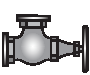
\includegraphics[scale=0.35]{../../figs/08HWEquivPipe/anglevalve} & Angle Valve & 150    \\
%        \midrule
%        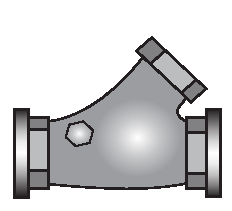
\includegraphics[scale=0.1]{../../figs/08HWEquivPipe/checkvalve}  & Check Valve & 100    \\
%        \midrule
%        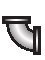
\includegraphics[scale=0.5]{../../figs/08HWEquivPipe/elbow}       & Elbow       & 50     \\
%        \midrule
%        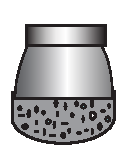
\includegraphics[scale=0.2]{../../figs/08HWEquivPipe/footvalve}   & Foot Valve  & 75     \\
%        \midrule
%        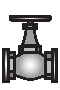
\includegraphics[scale=0.35]{../../figs/08HWEquivPipe/gatevalve}  & Gate Valve  & 35     \\
%        \bottomrule
%       \end{tabular}
%      \end{textblock*}
%
%      \begin{textblock*}{.35\textwidth}(6.5cm, 4cm)
%       \centering
%       \footnotesize
%       \begin{tabular}{cccc}
%        \toprule
%        Pipe & Length (m) & diam (mm) & C   \\
%        \midrule
%        AB   & 10         & 500       & 125 \\
%        \midrule
%        BC   & 2000       & 275       & 150 \\
%        \midrule
%        BD   & 1500       & 250       & 100 \\
%        \midrule
%        DC   & 1000       & 300       & 100 \\
%        \midrule
%        CE   & 10         & 500       & 125 \\
%        \bottomrule
%       \end{tabular}
%      \end{textblock*}
%
%
%     \end{frame}
%

\end{document}
